
\section{A Brief Introduction to VLBI}
\label{sec:vlbi}

We briefly describe VLBI to provide the necessary background for building an accurate likelihood model. Our goal is to provide intuition; for additional details 
%and derivations 
we recommend~\cite{thompson2008interferometry}.
%due to the inverse relationship between angular resolution and telescope diameter. 
As with cameras, a single-dish telescope is diffraction limited. 
%\delete{Diffraction imposes a fundamental limit on the minimum recoverable angular resolution of a $D$-diameter telescope observing at $\lambda$-wavelength to be $ \theta_{rad} \approx \lambda / D $.} 
However, simultaneously collecting data from an array of telescopes, called an interferometer, allows us to
%to decouple angular resolution from telescope diameter to 
overcome the single-dish diffraction limit. 
%The minimum angular resolution of an interferometer is inversely related to the maximum distance between telescopes. 



Figure~\ref{fig:introinterferometry} provides a simplified explanation of a two telescope interferometer. 
%Sinusoidal 
Electromagnetic radiation travels from a point source to the telescopes. However, because the telescopes are separated by a distance $B$, they will not receive the signal concurrently. 
%\footnote{This approximation is valid when the celestial emission being imaged is very far away as compared to the telescope baseline.}
For spatially incoherent extended emissions, the time-averaged correlation of the received signals is equivalent to the projection of this sinusoidal variation on the emission's intensity distribution.
%\footnote{ {\color{red}  Noise in the local atomic-clocks and baseline measurements are eliminated through a process called fringe searching that requires the use of a super-computer. }}


%Suppose we are observing a celestial point-source using two telescopes separated by a baseline vector $B$. Since the source is very far away, {\it both} telescopes are pointed at the source in the direction of the unit vector $\hat{s}$ and receive the same {\it plane-wave} signal. However, because the telescopes are separated by $B$ they will not receive the signals at the same time. 
%In Figure~\ref{fig:introinterferometry} we show geometrically that we can approximate the difference in the distance traveled to the telescopes as $ \Delta d  = B \cdot \hat{s} \label{eq:chdist} $. 
%Time-averaging the correlation of these phase-shifted signals results in a value that varies sinsoidally with the time delay. 
%For incoherant extended sources, it can be easily shown that the time-averaged correlation will be equivalent to the projection of this $\frac{B \cdot \hat{s}}{\lambda}$-frequency sinusoid on the source's spatial distribution. \katie{check this}


\begin{figure}[tb!]
	\centering
	{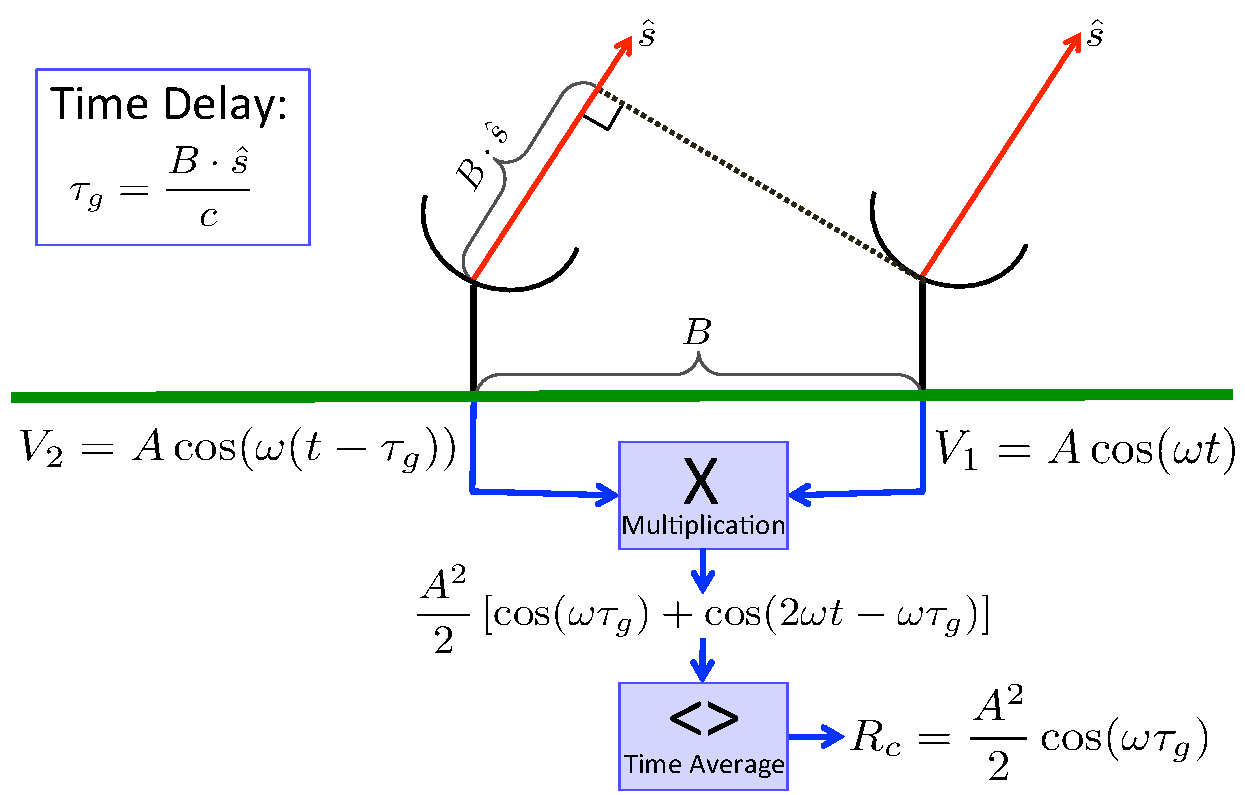
\includegraphics[width=\linewidth]
		{interferometryfig.pdf}}
	\caption{ \footnotesize{{\bf Simplified Interferometry Diagram:} 
			Light is emitted from a distant source and arrives at the telescopes as a plane wave in the direction $\hat{s}$. An additional distance of $B \cdot \hat{s}$ is necessary for the light to travel to the farther telescope, introducing  a time delay between the received signals that varies depending on the source's location in the sky. The time-averaged correlation of these signals is a sinusoidal function related to the location of the source. This insight is generalized to extended emissions in the van Cittert-Zernike Thm. and used to relate the time-averaged correlation to a Fourier component of the emission image in the direction $\hat{s}$.
			%Light of a single frequency is emitted from a point source and travels towards the telescopes. Since the point source is very far away, the telescopes point in the same direction, $\hat{s}$, and are hit by a plane wave. An additional distance of $B \cdot \hat{s}$ is necessary for the light to travel to the farther telescope. This extra distance introduces a time delay between the received signals. The time averaged correlation of these signals is then used to extract information about this delay. The time delay required for an emitted signal to reach the telescopes varies depending on the source location. We can use this insight to reconstruct an image of the emission.
			%\vspace{-.2in} 
			}}
	\label{fig:introinterferometry}
\end{figure}


%For incoherant extended sources, it can be shown that the time-averaged correlation of the signal from 2 telescopes is equivalent to the projection of a sinusoid on the source's spatial distribution. 
This phenomenon is formally described by the \textit{van Cittert-Zernike Theorem}. The theorem states that, for ideal sensors, the time-averaged correlation of the measured signals from two telescopes, $i$ and $j$, 
%seperated by a baseline, $B$, 
for a single wavelength, $\lambda$, can be approximated as:

\vspace{-.2in}
\begin{equation}  \Gamma_{i,j}(u,v) \approx \int_\ell{\int_{m} {e^{-i 2 \pi  (u\ell + vm) }} I_{\lambda}(\ell,m) dl} dm  \label{eq:visibility} \vspace{-.03in} \end{equation} 


\noindent{where $ I_{\lambda}(\ell,m)$ is the emission of wavelength $\lambda$ traveling from the direction  $\hat{s} = (\ell, m, \sqrt{1 - \ell^2 - m^2} )$. 
The dimensionless coordinates $(u,v)$ (measured in wavelengths) are the projected baseline, $B$, orthogonal to the line of sight.\footnote{The change in elevation between telescopes can be neglected due to corrections made in pre-processing. Additionally, for small FOVs wide-field effects are negligible.} Notice that Eq.~\ref{eq:visibility} is just the Fourier transform of the source emission image, $I_{\lambda}(\ell,m)$. Thus, $\Gamma_{i,j}(u,v)$
%\delete{the time-averaged correlation of the measured signals from two telescopes} 
provides a single complex Fourier component of $I_{\lambda}$ at position $(u,v)$ on the 2D spatial frequency plane. {\it We refer to these measurements, $\Gamma_{i,j}$, as visibilities.}
Since the spatial frequency, $(u,v)$, is proportional to the baseline, $B$, increasing the distance between telescopes increases the resolving power of the interferometer, allowing it to distinguish finer details. 


\vspace{-0.15in}
\paragraph{Earth Rotation Synthesis} At a single time, for an $N$ telescope array,
%, for every wavelength $\lambda$, 
%at a given time 
we obtain $ \frac{N(N-1)}{2} $ visibility measurements corresponding to each pair of telescopes. 
%we obtain measurements for $ \frac{N(N-1)}{2} $ constraints corresponding to the spatial frequency $(u,v)$ for each pair of telescopes. 
As the Earth rotates, the direction that the telescopes point towards the source ($\hat{s}$) changes. 
%Assuming a static source, this results in measuring different visibilities along elliptical paths in the $(u,v)$ frequency plane 
Assuming a static source, this yields measurements of spatial frequency components (visibilities) of the desired image along elliptical paths in the $(u,v)$ frequency plane (see Fig.~\ref{fig:uvcov}b). 
%Sampling $K$ times over the course of a day increases the number of frequency constraints $K$-fold.

\vspace{-0.15in}
\paragraph{Phase Closure} All equations thus far assumed that light travels from the source to a telescope through a vacuum. However, inhomogeneities in the atmosphere cause the light to travel at different velocities towards each telescope. These delays have a significant effect on the phase of measurements, and renders the phase unusable for image reconstructions at wavelengths less than 3 mm~\cite{monnier2013radio}. 

Although absolute phase measurements cannot be used, a clever observation - termed phase closure - allows us to still recover some information from the phases. 
The atmosphere affects an ideal visibility (spatial frequency measurement) by 
%The error due to the atmosphere for a single visibility measurement, 
introducing an additional phase term: $\Gamma_{i,j}^{\mbox{\tiny{meas}}} = e^{i(\phi_i - \phi_j)}\Gamma_{i,j}^{\mbox{\tiny{ideal}}}$,
%\begin{equation} \Gamma_{i,j}^{\mbox{\tiny{meas}}} = e^{i(\phi_i - \phi_j)}\Gamma_{i,j}^{\mbox{\tiny{ideal}}} \end{equation}
\noindent{where $\phi_i$ and $\phi_j$ are the phase delays introduced in the path to telescopes $i$ and $j$ respectively. By multiplying the visibilities from three different telescopes, we obtain an expression that is invariant to the atmosphere, as the unknown phase offsets cancel, see Eq.~\ref{eq:phaseclosure}~\cite{felli1989very}.  }

\vspace{-.2in}
\begin{align}  
\notag \Gamma^{\mbox{\tiny{meas}}}_{i,j}\Gamma^{\mbox{\tiny{meas}}}_{j,k}\Gamma^{\mbox{\tiny{meas}}}_{k,i} &= e^{i(\phi_i-\phi_j)}\Gamma^{\mbox{\tiny{ideal}}}_{i,j}e^{i(\phi_j-\phi_k)}\Gamma^{\mbox{\tiny{ideal}}}_{j,k}e^{i(\phi_k-\phi_i)}\Gamma^{\mbox{\tiny{ideal}}}_{k,i} \\
%= e^{i(\phi_i-\phi_j+\phi_j-\phi_k + \phi_k-\phi_i)}\Gamma^{\mbox{\tiny{true}}}_{i,j}\Gamma^{\mbox{\tiny{true}}}_{j,k}\Gamma^{\mbox{\tiny{true}}}_{k,i}  
&=\Gamma^{\mbox{\tiny{ideal}}}_{i,j}\Gamma^{\mbox{\tiny{ideal}}}_{j,k}\Gamma^{\mbox{\tiny{ideal}}}_{k,i} 
\label{eq:phaseclosure} 
 \end{align}
 


{\it We refer to this triple product of visibilities as the bispectrum}. The bispectrum is invariant to atmospheric noise; however, in exchange, it reduces the number of constraints that can be used in image reconstruction. Although the number of triple pairs in an $N$ telescope array is ${N\choose 3}$, the number of independent values is only $\frac{(N-1)(N-2)}{2}$.
%As $N$ becomes large, the ratio between the number of independent bispectrum values and the number of visibility measurements, $\frac{N(N-1)}{2}$, approaches unity.
%However, 
For small telescope arrays, such as the EHT, this effect is large. 
For instance, in an eight telescope array, using the bispectrum rather than visibilities results in 25\% fewer independent 
%bispectrum 
constraints 
%than visibilities
~\cite{felli1989very}.


%%\delete{Note how the phase delays perfectly cancel in the bispectrum. }
%{\it We refer to this triple product of visibilities as the bispectrum}. The bispectrum is invariant to a large amount of noise; 
%%on the other hand, 
%however, in exchange,
%%\katie{dont know if i like this change} 
%it reduces the number of constraints that can be used in image reconstruction. Although the number of triple pairs in an $N$ telescope array is ${N\choose 3}$, the number of independent values is only $\frac{(N-1)(N-2)}{2}$.
%As $N$ becomes large, the ratio between the number of independent bispectrum values and the number of visibility measurements, $\frac{N(N-1)}{2}$, approaches unity.
%However, for small telescope arrays, such as the EHT, the effect is large. 
%For instance, in an eight telescope array, this results in 25\% fewer independent 
%%bispectrum 
%constraints 
%%than visibilities
%~\cite{felli1989very}.


%However, for small telescope arrays, the effect is large. For instance, in a seven telescope array, there are only $15$ independent triple product measurements at a given time - this results in 28\% fewer independent bispectrum constraints when compared to the use of visibilities~\cite{felli1989very}.
 
\section{Related Work}
\label{sec:related}


 
%More BLAH however is the fact that absolute phase of VLBI Fourier measurements (visibilities) are lost due to atmospheric path delays. In SAR the Fourier samples are all coherantly related and the absolute phase can generally be recovered. However, 


%Note that this problem differs from traditional sparse spectral reconstruction methods (e.g MRI, CT) due to the large atmospheric phase errors. 

 %However, unlike in VLBI, 
 
 %Additionally, unlike in VLBI, traditional SAR and MRI are generally not plagued by large corruption of the signal's phase. High-resolution spaceborne SAR, on the other hand, does suffer from atmospheric path delays~\cite{atmosphereSAR}, which could be partially alleviated by modifying the system and incorporating phase closure in imaging, as is done in this work.

%multiple platforms into one super sar

%SAR sampling pattern is determined by trajectory of the pattern 
%typically measurements are made along a straight line

%SAR typically has uniform sampling of 
%In SAR resolves objects in range andn cross range where range is distance from antenna and range i perpendicular
%using conventuall sar with repeating chip (ie linear freq modulation ) waveforms you get a uniform sampling grid in spatial frequency corresponding to the range and cross range directions. 

%but more importantly those samples in the fourier domain are all coherantly related and the absolute phase can generally be recovered

%In there is an application with SAR there is no phase 

%the measurments in the Fourier space are all relatively coherant so you can do inverse 




%VLBI image reconstruction shares a lot in common with other sparse spectral image reconstruction problems, such as Synthetic Aperture Radar (SAR) and Magnetic Resonance Imaging (MRI)~\cite{bracewell2004fourier, compressedSAR}. In particular, although very different in practice, SAR is based on many of the same core ideas. 
%However, VLBI faces unique challenges that are not sufficiently addressed in these other fields.  %explored/
%For instance, the sampling of an image's Fourier plane is limited by the number and location of viable telescopes, whereas SAR and MRI both have much more flexibility in densely and uniformly sampling the plane. 
%Additionally, unlike in VLBI, traditional SAR and MRI are generally not plagued by large corruption of the signal's phase.  
%High-resolution spaceborne SAR on the other hand does suffer from atmospheric path delays~\cite{atmosphereSAR} that could be partially alleviated by modifying the system and incorporating phase closure in imaging, as is done in this work.


%However, the correction of atmospheric path delays in spaceborn SAR has become increasingly important 



%http://www.geo.uzh.ch/microsite/rsl-documents/research/publications/peer-reviewed-articles/sensors-08-08479-0152375552/sensors-08-08479.pdf
%http://www.geo.uzh.ch/microsite/rsl-documents/research/SARlab/Publications/PDF/JFS+04_poster.pdf

%http://download.springer.com/static/pdf/100/chp%253A10.1007%252F978-3-642-38398-4_13.pdf?originUrl=http%3A%2F%2Flink.springer.com%2Fchapter%2F10.1007%2F978-3-642-38398-4_13&token2=exp=1460032536~acl=%2Fstatic%2Fpdf%2F100%2Fchp%25253A10.1007%25252F978-3-642-38398-4_13.pdf%3ForiginUrl%3Dhttp%253A%252F%252Flink.springer.com%252Fchapter%252F10.1007%252F978-3-642-38398-4_13*~hmac=ad1ca5fad5ffee145885e5a423b3c4d472973f49766b40eb8fdcceff802d26b0

%The correction of atmospheric path delays in high-resolution spaceborne synthetic aperture radar systems has become increasingly important with continuing improvements to the resolution of SAR systems surveying the Earth. Atmospheric path delays must be taken into account in order to achieve geolocation accuracies better than 1 meter. These effects are mainly due to ionospheric and tropospheric influences. 

We summarize a few significant algorithms from the astronomical interferometry imaging literature.

%Image reconstruction from VLBI data has been studied for decades. We summarize a few significant algorithms.
%Reconstructing images from VLBI data has been an active field of research for some time. %decades. 
%While it is out of this paper's scope to provide a full survey of current literature, we summarize a few significant algorithms.
%present a brief summary of a few representative algorithms.


%\delete{ most applicable to VLBI image reconstruction.}

\vspace{-.15in}
\paragraph{CLEAN}

CLEAN is the de-facto standard method used for VLBI image reconstruction. It assumes that the image is made up of a number of bright point sources. From an initialization image, CLEAN iteratively looks for the brightest point in the image and ``deconvolves" around that location by removing side lobes that occur due to sparse sampling in the $(u,v)$ frequency plane. After many iterations, the final image of point sources is blurred~\cite{hogbom1974aperture}. Since CLEAN assumes a distribution of point sources, it often struggles with reconstructing images of extended emissions~\cite{taylor1999synthesis}.


For mm/sub-mm wavelength VLBI, reconstruction is complicated by corruption of the visibility phases. CLEAN is not inherently capable of handling this problem; however, self-calibration methods have been developed to greedily recover the phases during imaging. Self-calibration requires manual input from a knowledgeable user and often fails when the SNR is too low or the source is complex~\cite{taylor1999synthesis}. 


% CLEAN is the de-facto standard method used for VLBI image reconstruction. It works under the assumption that the image is made up of a number of bright point sources. Starting from an initialization, CLEAN iteratively looks for the brightest point in the image and ``deconvolves" around that location by removing side lobes that occur due to sparse sampling in the $(u,v)$ frequency plane. After many iterations, the final image is then blurred to de-emphasize spurious high frequencies~\cite{hogbom1974aperture}. Since CLEAN assumes a distribution of bright point sources, it often struggles with reconstructing images containing extended emissions~\cite{taylor1999synthesis}.

%For short-wavelength VLBI, reconstruction is complicated by the corruption of phase in visibility measurements. CLEAN is not inherently capable of handling this problem; however, self-calibration methods have been developed to greedily iterate back and forth between CLEANing the image and solving for closure constraints. Self-calibration requires manual input from a knowledgeable user and often fails when the SNR is too low or the source is complex~\cite{taylor1999synthesis}. 

%Although CLEAN is over 35 years old, theoretical understanding of the algorithm is limited. Success using CLEAN generally requires the use of many tricks and manual parameter tuning - especially in the case of self-calibration. Additionally, since it assumes a distribution of bright point sources, it struggles with reconstructing images containing extended emissions

 

\vspace{-.15in}
\paragraph{Optical Interferometry} 
Interferometry at visible wavelengths faces the same phase-corruption challenges as mm/sub-mm VLBI. %Therefore, in recent years a number of algorithms have been developed to try to reconstruct images under these conditions. 
Although historically the optical and radio interferometry communities have been separate, fundamentally the resulting measurements and imaging process are very similar~\cite{monnier2013radio}. 
We have selected two optical interferometry reconstruction algorithms representative of the field to discuss and compare to in this work~\cite{rusenimaging}. Both algorithms take a regularized maximum likelihood approach and can use the bispectrum, rather than visibilities, for reconstruction~\cite{baron2010novel, buscher1994direct}. Recent methods based on compressed sensing have been proposed, but have yet to demonstrate superior results~\cite{compressedsensing, rusenimaging}. 
%\footnote{Recent methods based on compressed sensing have yet to demonstrate superior results. CITATION}

%Interferometry at visible wavelengths faces the same phase-corruption challenges as mm-wavelength VLBI. %Therefore, in recent years a number of algorithms have been developed to try to reconstruct images under these conditions. 
%Although historically the optical and radio interferometry communities have been separate due to large differences in the specifics of data collection, fundamentally the resulting measurements and imaging process are the same~\cite{monnier2013radio}. 
%We have selected two optical interferometry reconstruction algorithms representative of the field to discuss and compare to in this work~\cite{rusenimaging}. Both algorithms take a regularized maximum likelihood approach and use the bispectrum, rather than visibilities, for reconstruction~\cite{buscher1994direct, baron2010novel}. Recent methods based on compressed sensing have been proposed, but have yet to demonstrate superior results~\cite{rusenimaging, compressedsensing}. 
%%\footnote{Recent methods based on compressed sensing have yet to demonstrate superior results. CITATION}

 BSMEM (BiSpectrum Maximum Entropy Method) takes a Bayesian approach to image reconstruction~\cite{buscher1994direct}. Gradient descent optimization~\cite{skilling1990quantified} using a maximum entropy prior is used to find an optimal reconstruction of the image. 
 %While there are many choices for the entropy function, BSMEM uses the Gull and Skilling entropy measure~\cite{skilling1990quantified}, generally with a flat or Gaussian model prior. 
 %As the winner of the last BLAH optical interferomic beauty contents, BSMEM has been the most successful method in recent years. 
 Under a flat image prior BSMEM is often able to achieve impressive super-resolution results on simple celestial images. However, in Section~\ref{section:results} we demonstrate how it often struggles on complex, extended emissions.
 %, which are believed to be present around black holes~\cite{fish2014imaging}.
 %extended emissions such as one expects to see around black holes.


% BSMEM (BiSpectrum Maximum Entropy Method), like our proposed algorithm, takes a Bayesian approach to image reconstruction~\cite{buscher1994direct}. Gradient descent optimization~\cite{skilling1990quantified} using a maximum entropy prior is used to find an optimal reconstruction of the image. While there are many choices for the entropy function, BSMEM uses the Gull and Skilling entropy measure~\cite{skilling1990quantified}, generally with a flat or Gaussian model prior. 
% %As the winner of the last BLAH optical interferomic beauty contents, BSMEM has been the most successful method in recent years. 
% Under a flat image prior BSMEM is often able to achieve impressive super-resolution results on simple celestial images. However, in Section~\ref{section:results} we demonstrate how it often struggles on complex, extended emissions, which are believed to be present around black holes~\cite{fish2014imaging}.
% %extended emissions such as one expects to see around black holes. 


SQUEEZE takes a Markov chain Monte Carlo (MCMC) approach to sample images from a posterior distribution~\cite{baron2010novel}. To obtain a sample image, SQUEEZE moves a set of point sources around the field of view (FOV). The final image is then calculated as the average of a number of sample images. 
Contrary to gradient descent methods, SQUEEZE is not limited in its choice of regularizers or constraints~\cite{rusenimaging}. 
%Additionally, under a specified set of parameters, given enough time, the algorithm is guaranteed to find the distribution's expected image. 
However, this freedom comes at the cost of a large number of parameter choices that may be hard for an unknowledgeable user to select and tune. 

%SQUEEZE takes a Markov chain Monte Carlo (MCMC) approach to sample images from a posterior probability distribution~\cite{baron2010novel}. To obtain a sample image, SQUEEZE moves a set of point sources around the field of view (FOV) until a maximum number of iterations has been reached. The final image is then calculated as the mean of a chosen number of sample images. 
%Contrary to gradient descent methods, SQUEEZE is not limited in its choice of regularizers or constraints~\cite{rusenimaging}. Additionally, under a specified set of parameters, given enough time, the algorithm is guaranteed to find the distribution's expected image. However, this freedom comes at the cost of a large number of parameter choices that may be hard for an unknowledgable user to select and tune. 

\subsection{Spectral Image Reconstruction}

VLBI image reconstruction has similarities with other spectral image reconstruction problems, such as Synthetic Aperture Radar (SAR), Magnetic Resonance Imaging (MRI), and Computed Tomography (CT)~\cite{bracewell2004fourier, lustig2007sparse, 1456966, thibault2007three}. %, although a detailed comparison is beyond the scope of this work
However, VLBI faces a number of challenges that are typically not relevant in these other fields. % (e.g. sampling limits, SNR). 
%For instance, in VLBI the sampling of an image's Fourier plane is limited by the number and location of viable telescopes, whereas other methods typically have more flexibility in densely and uniformly sampling the Fourier plane. 
For instance, SAR, MRI, and CT are generally not plagued by large corruption of the signal's phase, as is the case due to atmospheric differences in mm/sub-mm VLBI. In SAR the Fourier samples are all coherently related and the absolute phase can generally be recovered, even under atmospheric changes~\cite{533208, 6504845}. However, although fully understanding the connection remains an open problem, incorporating ideas of phase closure, as is done in this work, may open the potential to push SAR techniques~\cite{atmosphereSAR} past their current limits.
